%%%%%%%%%%%%%%%
%%
%%						SEMANTIC PHASE / HASH-CONSING
%%
%%%%%%%%%%%%%%%%%%%%%%%%%%%%%%%%%%%%%%%%%%%%%%%%%%%%%%%%%%%%%%%%%%%%%%%%%%%%%%%%%%%
%%%%%%%%%%%%%%%%%%%%%%%%%%%%%%%%%%%%%%%%%%%%%%%%%%%%%%%%%%%%%%%%%%%%%%%%%%%%%%%%%%%



%----------------------------------------------------------------------------------
\begin{frame}{The Semantic Phase}{Hash-consing}
%----------------------------------------------------------------------------------
The Faust compiler heavily relies on \emph{hash-consing} to discover common sub-expressions, and on \emph{memoization} to speedup compilation. 
\begin{eqnarray*}
T_1=T_2 &\Rightarrow& \mathsf{Addr}(T_1)=\mathsf{Addr}(T_2)\\
\mathsf{Addr}(T_1)\neq\mathsf{Addr}(T_2) &\Rightarrow& T_1\neq T_2 
\end{eqnarray*}

Problem : Hash-consing can miss potential sharings. Simplification and normalization are used to improve sharing and common subexpression elimination.

\end{frame}


%----------------------------------------------------------------------------------
\begin{frame}{The Semantic Phase}{Hash-consing}
%----------------------------------------------------------------------------------

Miss due to associativity or commutativity :

\begin{columns}
\column{.5\textwidth}
\begin{center}\begin{tikzpicture}[scale=.7]
\Tree [.\expr'*' \expr'<<A>>' [.\expr'*' \expr'<<B>>'  \expr'<<C>>' ] ]
\end{tikzpicture}\end{center}
\column{.5\textwidth}
\begin{center}\begin{tikzpicture}[scale=.7]
\Tree [.\expr'*' \expr'<<A>>' \expr'<<C>>' ]
\end{tikzpicture}\end{center}
\end{columns}

Miss due to $\alpha-$equivalence :

\begin{columns}
\column{.5\textwidth}
\begin{center}\begin{tikzpicture}[scale=.7]
\Tree [.\expr'REC[<<x>>]' [.\expr'+' \expr'IN[0]' [.\expr'@' \expr'PROJ[<<x>>][0]'  1 ] ] ]
\end{tikzpicture}\end{center}
\column{.5\textwidth}
\begin{center}\begin{tikzpicture}[scale=.7]
\Tree [.\expr'REC[<<y>>]' [.\expr'+' \expr'IN[0]' [.\expr'@' \expr'PROJ[<<y>>][0]'  1 ] ] ]
\end{tikzpicture}\end{center}
\end{columns}

\end{frame}


%----------------------------------------------------------------------------------
\begin{frame}{The Semantic Phase}{Simplification and normalization}
%----------------------------------------------------------------------------------
Polynomial expressions are rewritten as sum of products : $k_1A^mB^n\ldots + k_2C^iD^j\ldots$ and then factorized.

\begin{eqnarray*}
0*A &\rightarrow& 0\\
1*A &\rightarrow& A\\
A*k &\rightarrow& k*A\\
(k*A)*(k'*B)  &\rightarrow& (k*k')*(A*B)\\
B*A  &\rightarrow& A*B\\
A^n*A^m  &\rightarrow& A^{n+m}\\
0+A  &\rightarrow& A \\
B+A  &\rightarrow& A+B \\
A*B+A*C  &\rightarrow& A*(B+C)
\end{eqnarray*}

\end{frame}


%----------------------------------------------------------------------------------
\begin{frame}{The Semantic Phase}{Simplification and normalization}
%----------------------------------------------------------------------------------
Example  : $4y+2xy+3xyz \rightarrow y(4+x(2+3z))$

\begin{columns}
\column{.5\textwidth}
\Tree [.+ [.* 4 y ] [.+ [.* 2 [.* x y ] ] [.* 3 [.* y [.* z x ] ] ] ] ]

\column{.5\textwidth}
\Tree [.* y [.+ 4 [.* x [.+ 2 [.* 3 z ] ] ] ] ]
\end{columns}

\end{frame}


%----------------------------------------------------------------------------------
\begin{frame}{The Semantic Phase}{Simplification and normalization}
%----------------------------------------------------------------------------------
Reorganization of delay lines moved towards inputs :


\begin{eqnarray*}
0z^{-n} &\rightarrow& 0\\
Az^{0} &\rightarrow& A\\
(k*A)z^{-n} &\rightarrow& k*Az^{-n}\\
Az^{-n}z^{-m} &\rightarrow& Az^{-(n+m)}
\end{eqnarray*}

\end{frame}


%----------------------------------------------------------------------------------
\begin{frame}{The Semantic Phase}{Sharing of recursive terms}
%----------------------------------------------------------------------------------

\emph{Problem with hash-consing} : $\alpha-$equivalent recursive terms in standard notation are not shared:

\begin{columns}
\column{.5\textwidth}
\begin{center}\begin{tikzpicture}[scale=.7]
\Tree [.\expr'REC[<<x>>]' [.\expr'+' \expr'IN[0]' [.\expr'@' \expr'PROJ[<<x>>][0]'  1 ] ] ]
\end{tikzpicture}\end{center}
\column{.5\textwidth}
\begin{center}\begin{tikzpicture}[scale=.7]
\Tree [.\expr'REC[<<y>>]' [.\expr'+' \expr'IN[0]' [.\expr'@' \expr'PROJ[<<y>>][0]'  1 ] ] ]
\end{tikzpicture}\end{center}
\end{columns}

\vspace{0.25cm}
Open terms in de Bruijn notation are incorrectly shared:
 
\begin{columns}
\column{.5\textwidth}
\begin{center}\begin{tikzpicture}[scale=.7]
\Tree [.\expr'REC[]' [.\expr'+' \expr'IN[0]' [.\expr'@' \expr'PROJ[0][0]'  1 ] ] ]
\end{tikzpicture}\end{center}
\column{.5\textwidth}
\begin{center}\begin{tikzpicture}[scale=.7]
\Tree [.\expr'REC[]' [.\expr'+' \expr'1' [.\expr'@' \expr'PROJ[0][0]'  1 ] ] ]
\end{tikzpicture}\end{center}
\end{columns}

\end{frame}


%----------------------------------------------------------------------------------
\begin{frame}[fragile]{The Semantic Phase}{Sharing of recursive terms}
%----------------------------------------------------------------------------------

\emph{Solution} : start in de Bruijn notation and progressively transform de Bruijn terms into standard terms.
\vspace{0.25cm}

\begin{columns}
\column{.5\textwidth}
\begin{center}\begin{tikzpicture}[scale=.45]
\Tree [.\expr'REC[]' [.\expr'+' [.\expr'REC[]' [.\expr'+' \expr'IN[0]' [.\expr'+'  [.\expr'@' \expr'PROJ[0][0]'  1 ] [.\expr'@' \expr'PROJ[1][0]'  1 ] ] ] ]  [.\expr'@' \expr'PROJ[0][0]'  1 ] ] ]
\end{tikzpicture}\end{center}

\column{.5\textwidth}
\begin{center}\begin{tikzpicture}[scale=.45]
\Tree [.\expr'REC[x]' [.\expr'+' [.\expr'REC[]' [.\expr'+' \expr'IN[0]' [.\expr'+'  [.\expr'@' \expr'PROJ[0][0]'  1 ] [.\expr'@' \expr'PROJ[x][0]'  1 ] ] ] ]  [.\expr'@' \expr'PROJ[x][0]'  1 ] ] ]
\end{tikzpicture}\end{center}

\end{columns}
\begin{center}\begin{tikzpicture}[scale=.45]
\Tree [.\expr'REC[x]' [.\expr'+' [.\expr'REC[y]' [.\expr'+' \expr'IN[0]' [.\expr'+'  [.\expr'@' \expr'PROJ[y][0]'  1 ] [.\expr'@' \expr'PROJ[x][0]'  1 ] ] ] ]  [.\expr'@' \expr'PROJ[x][0]'  1 ] ] ]
\end{tikzpicture}\end{center}

\end{frame}



%----------------------------------------------------------------------------------
\begin{frame}[fragile]{The Semantic Phase}{Type Annotation and interval computation}
%----------------------------------------------------------------------------------
Signals are annotated with various information used to guide the code generation :

\begin{itemize}
\item \emph{nature}: integer or floating point values
\item \emph{boolean}: when a signal stands for a boolean value
\item \emph{variability}: how fast values change (constant, at each block or at each sample)
\item \emph{computability}: when values are available (at compile time, at initialization time, at execution time)
\item \emph{vectorability}: when a signal computation can be vectorized
\item \emph{interval}: minimal and maximal values a signal can take
\item \emph{occurrence context}: maximal delay, number of occurrences
\end{itemize}


\end{frame}



%----------------------------------------------------------------------------------
\begin{frame}[fragile]{The Semantic Phase}{Resulting signals for the Moog example}
%----------------------------------------------------------------------------------

\begin{figure}
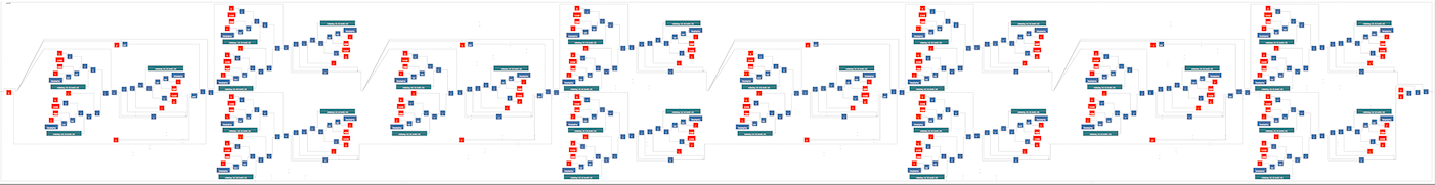
\includegraphics[width=1\columnwidth]{images/flat-moog-circuit}
\caption{Flat circuit after evaluation of the Faust program}
\end{figure}

\begin{figure}
\includegraphics[width=1\columnwidth]{images/moog-sig}
\caption{Resulting signal after symbolic propagation in the circuit and normalization}
\end{figure}


\end{frame}
